\documentclass[11pt,a4paper]{article}

\usepackage[utf8]{inputenc}
\usepackage[T1]{fontenc}
\usepackage{amsmath,amssymb}
\usepackage{geometry}
\usepackage{booktabs}
\usepackage{listings}
\usepackage{pgfplots}
\usepackage[colorlinks=true,linkcolor=blue,citecolor=blue,urlcolor=blue]{hyperref}

\geometry{left=2.5cm,right=2.5cm,top=2.5cm,bottom=2.5cm}
\pgfplotsset{compat=1.18}

\lstset{
  basicstyle=\ttfamily\small,
  breaklines=true,
  frame=single,
  numbers=left,
  numberstyle=\tiny,
  tabsize=2
}

\title{\textbf{NRR-Coupled (cp) v4: Dependency-Consistency Evaluation Without Tautological References}}
\author{Kei Saito\\Independent Researcher, Japan\\\texttt{kei.saito.research@gmail.com}}
\date{February 2026\\[0.5em]\textit{Part of the Non-Resolution Reasoning (NRR) research program.}}

\begin{document}
\maketitle

\begin{center}
\textcopyright\ 2026 Kei Saito. Licensed under CC BY 4.0.\\
\url{https://creativecommons.org/licenses/by/4.0/}
\end{center}

\begin{abstract}
cp v3 used a coupled-generated reference trajectory and was vulnerable to circular evaluation. This paper introduces cp v4, which removes that dependence and evaluates coupled propagation by dependency consistency itself. We keep the same fixed interface (LLM emits \((\sigma/\delta,\text{target})\); client executes updates) and compare uncoupled baseline (\(\beta=0\)) with coupled variants (\(\beta\in\{0.1,0.3,0.5\}\)). Evaluation uses 15 seed-fixed random operator streams for each of 3 patterns (\(n=4,5,6\)); each stream targets only primary candidates for 12 turns. Main metrics are (i) turn-wise dependency-consistency violation rate and (ii) additional repair operators needed after the primary stream. At \(\beta=0.3\), coupled updates reduce violation rate in D-dependent by 0.2123 and reduce repair operations by 0.58 on average, while D-mismatch increases violation rate by 0.2302 and repair operations by 3.31. D-independent remains exactly equivalent (tolerance \(10^{-12}\)). These results support a conditional claim: cp improves consistency only when dependency structure is correct and degrades under sign-mismatched dependencies.
\end{abstract}

\noindent\textbf{Keywords:} NRR-Coupled, dependency consistency, repair cost, falsifiable simulation, robustness

\section{Introduction}
LLM APIs are stateless across calls, while many applications require state updates over dependent candidates. NRR-Transfer addressed independent-candidate updates; cp extends client execution to dependent settings.

NRR is not an anti-LLM framework.
NRR does not replace standard LLM use.
NRR optimizes when to commit and when to defer, under explicit conditions.

\textbf{Boundary.}
Transfer: independent-candidate condition.
cp: dependent-candidate condition.
Uncoupled baseline is inherited from Transfer and not redefined.

\textbf{v4 motivation.}
To avoid circular scoring, v4 does not use coupled-generated reference states as evaluation targets. Instead, it measures whether produced transitions satisfy declared dependency relations.

Series Consistency Statement: Unsupported interpretations are never injected at a fixed evidence state. Hypothesis-set expansion is evidence-gated, and unobserved possibilities remain unresolved. Evidence in this paper is restricted to fixed simulation inputs and declared dependency structures.

\section{Update Rule and Complexity}
Let \(\mathbf{w}_t\in\mathbb{R}^n\), \(\sum_i w_t^{(i)}=1\), and dependency matrix \(A\in\mathbb{R}^{n\times n}\), where \(A_{ij}\) is influence from candidate \(j\) to \(i\).

Given \((o_t,k_t)\) with \(o_t\in\{\sigma,\delta\}\):
\[
\Delta_t = +\alpha\;(\sigma),\ -\alpha\;(\delta),\qquad
\tilde{w}^{(k_t)}=\operatorname{clip}(w_t^{(k_t)}+\Delta_t,\varepsilon,u_{\max}).
\]
\[
\tilde{w}^{(i)} \leftarrow \operatorname{clip}(\tilde{w}^{(i)}+\beta A_{i,k_t}(\tilde{w}^{(k_t)}-w_t^{(k_t)}),\varepsilon,u_{\max}),\ i\neq k_t.
\]
Renormalization is Transfer-compatible (target fixed, non-target proportional scaling).

Per-turn complexity (sparse):
\[
T_{\text{turn}}=O\big(n+\deg_{\text{out}}(k_t)\big),
\]
with naive full-matrix upper bound \(O(n^2)\).

\section{v4 Evaluation Design}
\subsection{Patterns and streams}
Patterns:
\begin{itemize}
  \item P1-n4 (\(n=4\), primary targets \(\{0,1\}\))
  \item P2-n5 (\(n=5\), primary targets \(\{0,1,2\}\))
  \item P3-n6 (\(n=6\), primary targets \(\{0,1,2\}\))
\end{itemize}
For each pattern, 15 seed-fixed random streams are generated, each 12 turns.
Operators are random \((\sigma/\delta,\text{target})\) pairs with targets restricted to primary candidates.

\subsection{Dependency conditions}
\begin{itemize}
  \item D-dependent: model matrix \(A_{\text{model}}=A_{\text{dep}}\), evaluation matrix \(A_{\text{eval}}=A_{\text{dep}}\)
  \item D-independent: \(A_{\text{model}}=A_{\text{eval}}=0\)
  \item D-mismatch: \(A_{\text{model}}=-A_{\text{dep}}\), \(A_{\text{eval}}=A_{\text{dep}}\)
\end{itemize}

Matrix generation:
\[
A_{(j+1)\bmod n,j}=p_n,\;
A_{(j+2)\bmod n,j}=q_n<0,\;
A_{(j-1)\bmod n,j}=s_n,
\]
others zero, with
\((p_4,q_4,s_4)=(1.20,-0.90,0.70)\),
\((p_5,q_5,s_5)=(1.10,-0.80,0.65)\),
\((p_6,q_6,s_6)=(1.00,-0.75,0.60)\).

\subsection{Compared systems}
\begin{itemize}
  \item baseline uncoupled: \(\beta=0\)
  \item coupled cp: \(\beta\in\{0.1,0.3,0.5\}\)
\end{itemize}

\section{Metrics}
\subsection{M1: turn-wise dependency-consistency violation rate}
For each turn with operation sign \(s_t\in\{+1,-1\}\) and target \(k_t\), for every edge \(i\leftarrow k_t\) with \(A_{\text{eval},i,k_t}\neq 0\), expected sign is
\[
\operatorname{sign}(\Delta w_t^{(i)}) = \operatorname{sign}(A_{\text{eval},i,k_t})\cdot s_t.
\]
A violation is counted when observed sign contradicts the expected sign (beyond tolerance).
Violation rate is total violations divided by total opportunities.

\subsection{M2: additional repair operator count}
After the primary stream, we run greedy repair on non-primary candidates.
For each dependent candidate \(i\), signal is
\[
\text{signal}_i = \sum_{j\in\text{primaries}} A_{\text{eval},i,j}(w_j-w_{0,j}).
\]
If candidate shift \((w_i-w_{0,i})\) has opposite sign to \(\text{signal}_i\), it is a mismatch.
Greedy repair applies \(\sigma\) or \(\delta\) to the largest mismatch until no mismatch remains or max-repair budget is reached.

\subsection{Pairwise deltas}
For each sample:
\[
\Delta V = V_{cp} - V_{base},\qquad
\Delta R = R_{cp} - R_{base},
\]
where \(V\) is violation rate and \(R\) is repair-op count.
Negative values indicate cp improvement.

\section{Falsifiable Criteria (\(\beta=0.3\))}
\begin{enumerate}
  \item D-dependent: mean \(\Delta V < 0\)
  \item D-dependent: mean \(\Delta R < 0\)
  \item D-mismatch: mean \(\Delta V > 0\) and mean \(\Delta R > 0\)
  \item D-independent: mean deltas are non-negative baseline-equivalent and strict equality check passes at \(10^{-12}\)
\end{enumerate}

\section{Results}
Samples per condition and beta: \(3\) patterns \(\times\) \(15\) streams = \(45\).

\begin{center}
\begin{tabular}{@{}llcc@{}}
\toprule
Condition & Metric (\(\beta=0.3\)) & Mean $\pm$ SD & Min / Max \\
\midrule
D-dependent & $\Delta V$ & $-0.2123 \pm 0.0857$ & $-0.4167 / 0.0000$ \\
D-dependent & $\Delta R$ & $-0.5778 \pm 0.8561$ & $-3 / 2$ \\
D-independent & $\Delta V$ & $0.0000 \pm 0.0000$ & $0.0000 / 0.0000$ \\
D-independent & $\Delta R$ & $0.0000 \pm 0.0000$ & $0 / 0$ \\
D-mismatch & $\Delta V$ & $0.2302 \pm 0.0669$ & $0.0833 / 0.3333$ \\
D-mismatch & $\Delta R$ & $3.3111 \pm 6.9051$ & $-2 / 28$ \\
\bottomrule
\end{tabular}
\end{center}

\begin{figure}[t]
\centering
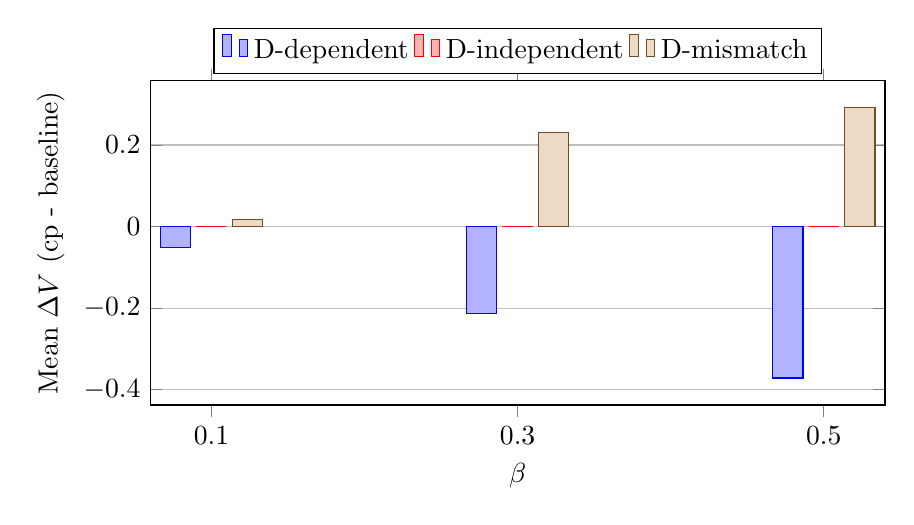
\begin{tikzpicture}
\begin{axis}[
  ybar,
  bar width=11pt,
  width=0.9\textwidth,
  height=5.7cm,
  xlabel={$\beta$},
  ylabel={Mean $\Delta V$ (cp - baseline)},
  symbolic x coords={0.1,0.3,0.5},
  xtick=data,
  legend style={at={(0.5,1.02)},anchor=south,legend columns=3},
  ymajorgrids=true
]
\addplot coordinates {(0.1,-0.0506) (0.3,-0.2123) (0.5,-0.3716)};
\addplot coordinates {(0.1,0.0000) (0.3,0.0000) (0.5,0.0000)};
\addplot coordinates {(0.1,0.0167) (0.3,0.2302) (0.5,0.2914)};
\legend{D-dependent,D-independent,D-mismatch}
\end{axis}
\end{tikzpicture}
\caption{Mean violation-rate difference across 45 samples per condition and beta.}
\label{fig:vdiff_v4}
\end{figure}

\begin{figure}[t]
\centering
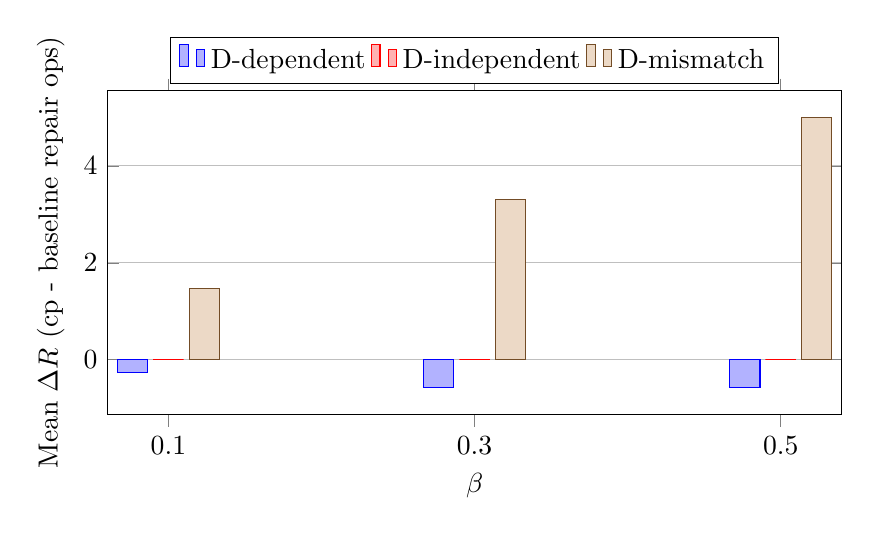
\begin{tikzpicture}
\begin{axis}[
  ybar,
  bar width=11pt,
  width=0.9\textwidth,
  height=5.7cm,
  xlabel={$\beta$},
  ylabel={Mean $\Delta R$ (cp - baseline repair ops)},
  symbolic x coords={0.1,0.3,0.5},
  xtick=data,
  legend style={at={(0.5,1.02)},anchor=south,legend columns=3},
  ymajorgrids=true
]
\addplot coordinates {(0.1,-0.2667) (0.3,-0.5778) (0.5,-0.5778)};
\addplot coordinates {(0.1,0.0000) (0.3,0.0000) (0.5,0.0000)};
\addplot coordinates {(0.1,1.4667) (0.3,3.3111) (0.5,5.0000)};
\legend{D-dependent,D-independent,D-mismatch}
\end{axis}
\end{tikzpicture}
\caption{Mean repair-op difference across 45 samples per condition and beta.}
\label{fig:rdiff_v4}
\end{figure}

\subsection{Pass/fail}
From `cp\_v4\_report.json` at \(\beta=0.3\): all criteria pass.
D-dependent improves on both metrics; D-mismatch degrades on both metrics; D-independent remains exactly equivalent.

\section{Discussion}
v4 resolves the circular-reference problem by scoring consistency directly from declared dependencies, not from coupled-generated target states. Under this design, cp remains conditionally useful and clearly falsifiable: wrong dependency signs produce measurable degradation.

\section{Reproducibility}
Artifacts:
\begin{itemize}
  \item `spec/nrr-coupled\_spec\_v4.md`
  \item `repro/coupled\_state\_sim.py`
  \item `repro/README\_v4.md`
  \item `repro/results/cp\_v4\_*.csv`
  \item `repro/results/cp\_v4\_report.json`
\end{itemize}

Main run:
\begin{lstlisting}
python3 repro/coupled_state_sim.py --outdir repro/results
\end{lstlisting}

\begin{thebibliography}{9}
\bibitem{saito2025nrr}
Saito, K. (2025).
\textit{NRR-Core: Non-Resolution Reasoning as a Computational Framework for Contextual Identity and Ambiguity Preservation}.
arXiv:2512.13478.

\bibitem{saito2026phi}
Saito, K. (2026).
\textit{NRR-Phi: Text-to-State Mapping for Ambiguity Preservation in LLM Inference}.
arXiv:2601.19933.

\bibitem{saito2026transfer}
Saito, K. (2026).
\textit{NRR-Transfer: Cross-Domain Transfer of Phase 1.5 Operators Under Fixed Interface Constraints}.
Manuscript v30 (pre-submission line).
\end{thebibliography}

\end{document}
